% I suggest we discuss briefly Timepix detectors use on the ISS and other places for space radiation dosimetry and particle identification. We can also talk a bit about our motivations of studying cosmic rays on commercial airline flights.

\section{Background}
\label{Background}

TimePIX detectors have many applications in the realm of Particle Physics. 
%
Numerous balloon flights have included the use of TimePIX devices for the purposes of particle imaging and radiation dosimetry in unusual and unfamiliar environments, such as the stratosphere \cite{bexus}. 
%
The International Space Station (ISS) uses TimePIX devices to evalute the astronauts' exposure to ionizing radiation fields \cite{timepixiss}.
%below is an actual space

The TimePIX device used in this flight was a MiniPIX, which is a silicon-based hybrid pixel detector built by ADVACAM \cite{advacam}. 
%
The sensor surface offers a resolution of 256x256 pixels.
%
The device can be operated under one of three modes: time-of-arrival (TOA) or time-over-threshold (TOT), or single particle counting. 
%
When a particle ionizes with the silicon chip, the deposited charge is depleted by a bias voltage in a process known as Carrier generation and recombination. \textbf{<<Verify the previous statement>>}
%below is an actual space

\begin{figure}[h]
    \centering
    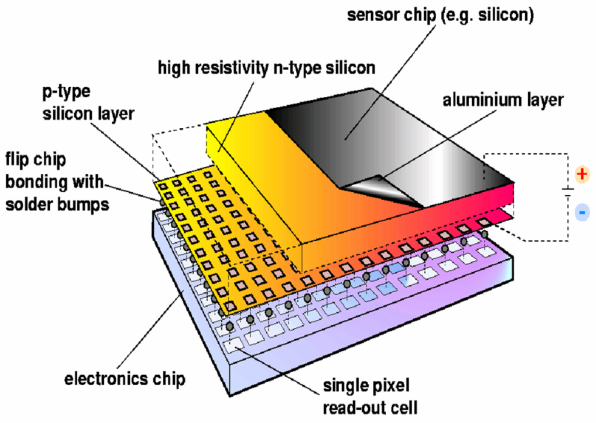
\includegraphics[width=0.25\textwidth]{minipix_silicon.pdf}
    \caption{MiniPIX silicon concept design}
    \label{fig:minipix_silicon}
\end{figure}
%

\textbf{<<Include silicon-chip figure?>>}
%figure name: minipix_silicon.pdf
